\chapter{The Bouc-Wen Model of Hysteresis}
\label{app:bouc-wen}

A hysteretic semi-physical model has been initially proposed by Bouc
in 1971~\cite{bouc} and subsequently generalized by Wen in 1976~\cite{bouc_wen}.
Since then, it was known as the Bouc-Wen model and 
as been extensively used in the current literature to describe
mathematically components and devices with hysteretic behaviours,
particularly within the areas of civil and mechanical engineering.


\begin{wrapfigure}{l}{0.6\textwidth}
	\centering
	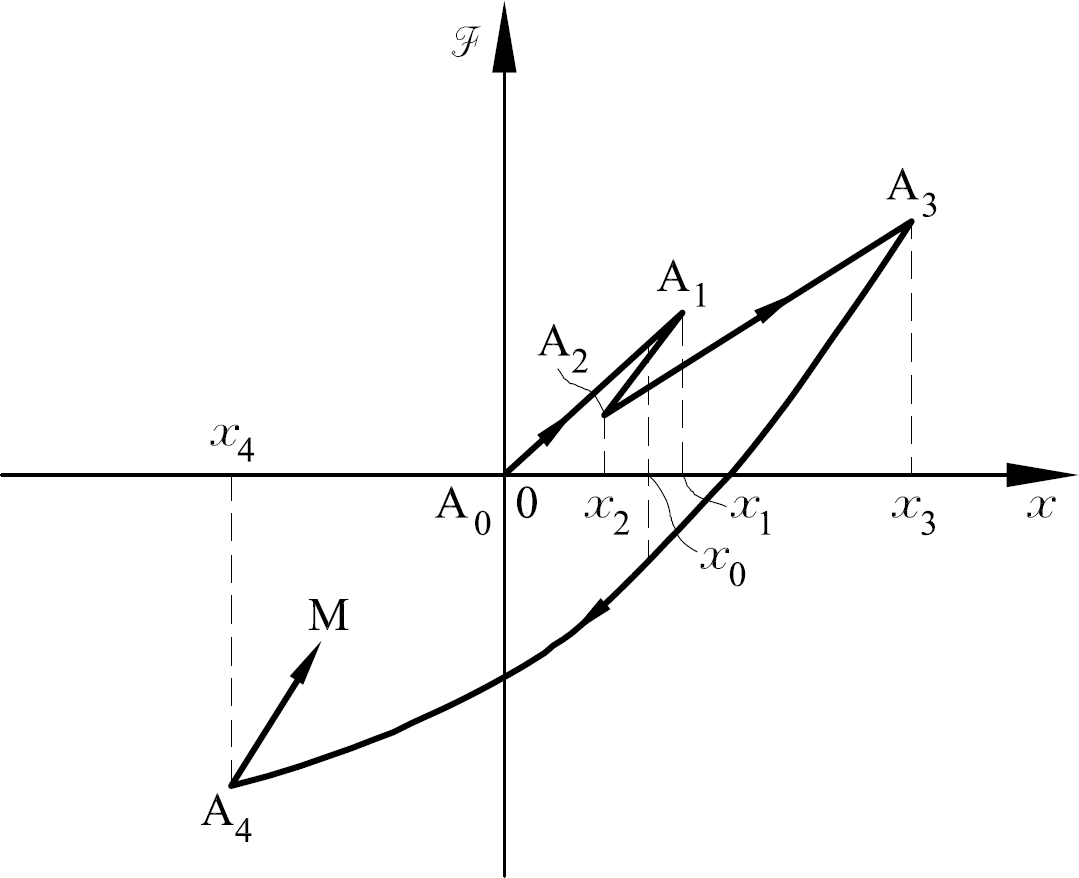
\includegraphics[width=.6\textwidth]{Images/functional}
	\caption{Graph force versus displacement for a hysteresis functional}
	\label{fig:functional}
\end{wrapfigure}

The model consists of a first-order non-linear differential equation
that relates the input displacement to the output restoring
force in a hysteretic way. By choosing a set of parameters
appropriately, it is possible to accommodate the response of
the model to the real hysteresis loops.

In the first paper by Bouc, a functional that describes
the hysteresis phenomenon was proposed. Given $\mathcal{F}$ a force
and $x$ a displacement, from Figure~\ref{fig:functional}
it can be seen that four values of $\mathcal{F}$ correspond
to the single point $x = x_0$. If we consider that $x$ is a function of time,
then the value of the force at instant time $t$ depends not only
from the value of the displacement $x$ at time $t$, but also on past values of $x$.

The following simplifying assumption is made in the original paper.

\newtheorem{assumption1}{Assumption}[chapter]

\begin{assumption1} \label{ass:rip}
The graph of Figure~\ref{fig:functional} remains the same for all
increasing function $x(\cdot)$ between $0$ and $x_1$, for all decreasing
function $x(\cdot)$ between the values $x_1$ and $x_2$, etc.
\end{assumption1}

In current literature, Assumption~\ref{ass:rip} is referred to as
the \emph{rate-independent property}~\cite{visintin2013differential}.
In his paper, Bouc proposes Equation~\ref{eq:functional} as a form for $\mathcal{F}$.

\begin{align} \label{eq:functional}
\frac{d\mathcal{F}}{dt} = g \left(x,\mathcal{F},\sign\left(\frac{dx}{dt}\right)\right)\frac{dx}{dt}.
\end{align}

Consider the equation

\begin{align} \label{eq:functional2}
\frac{d^2x}{dt^2}+\mathcal{F}\left(t\right) = p\left(t\right)
\end{align}

for some given input $p\left(t\right)$ and initial conditions

\begin{align}
\frac{dx}{dt}\left(t_0\right),\qquad x\left(t_0\right)\quad \text{and}\quad \mathcal{F}\left(t_0\right)
\end{align}

at the initial time $t_0$. Equations~\ref{eq:functional} and~\ref{eq:functional2}
describe completely a hysteretic oscillator. Since it is difficult to explicitly
find a solution for Equation~\ref{eq:functional} due to the nonlinearity of the
function $g$, Bouc proposes a variation of the Stieltjes integral to define $\mathcal{F}$:

\begin{align}
\mathcal{F}\left(t\right) = \mu^2x\left(t\right)+\int_\beta^tF\left(V_s^t\right)dx\left(s\right)
\end{align}

where $\beta \in \left[-\inf,+\inf\right)$ is the time instant after which
the displacement and force are defined. $V_s^t$ is the total variation of $x$
in the time interval $\left[s,t\right]$. The function F is chosen so that it
satisfies mathematical properties compatible with the hysteresis. In his work,
Bouc chooses the function F in Equation~\ref{eq:bouc_chosen}:

\begin{align} \label{eq:bouc_chosen}
F\left(u\right)= \sum_{i=1}^N A_i e^{-\alpha_iu},\quad \text{with } \alpha_i > 0
\end{align}

Using this result, Equations~\ref{eq:functional2}--\ref{eq:bouc_chosen}
can be rewritten in the following form.

\begin{align}\label{eq:bouc1}
\frac{d^2x}{dt^2} + \mu^2x + \sum_{i=1}^NZ_i=p\left(t\right)
\end{align}
\begin{align}\label{eq:bouc2}
\frac{dZ_i}{dt} + \alpha_i \left|\frac{dx}{dt}\right|Z_i - A_i\frac{dx}{dt}=0,\quad i=1,\dots,N
\end{align}

Equations~\ref{eq:bouc1} and~\ref{eq:bouc2} are known as the Bouc model.
Equation~\ref{eq:bouc2} has been extended by Wen to describe the restoring
forces with hysteresis in the following form:

\begin{align}
&\dot{z} = A\dot{x} - \alpha\left|\dot{x}\right|z^n - \beta \dot{x}\left|z^n\right| & & \text{for n odd} \label{eq:bw_1} \\
&\dot{z} = A\dot{x} - \alpha\left|\dot{x}\right|z^{n-1}\left|z\right| - \beta \dot{x}z^n & &\text{for n even} \label{eq:bw_2}
\end{align}

Equations~\ref{eq:bw_1} and \ref{eq:bw_2} are the earliest version of what
is known as the Bouc-Wen model of hysteresis.





















